%Dokumententyp
\documentclass[a4paper]{article}

\usepackage[a4paper,left=2cm, right=3cm, top=2cm]{geometry}

%Kodierung
\usepackage[utf8]{inputenc}
\usepackage[T1]{fontenc}

%Grafiken einbinden
\usepackage{graphicx}
\usepackage{subfigure} 

%Position von Grafiken und Tabellen erzwingen:
\usepackage{float}

%URLs im Literaturverzeichnis
\usepackage{url}

\usepackage{amsmath}

%Vektoren einfacher angeben:
\newcommand{\vektor}[1]{\left( \begin{array}{c} #1 \end{array} \right) }


%Schriftart Arial:
% \usepackage{helvet}

%Figures with text around it:
\usepackage{wrapfig}

\usepackage{listings}

%seitennummern rechts:
% \usepackage{fancyhdr}
% \fancyhf{} % clear all header and footers
% \renewcommand{\headrulewidth}{0pt} % remove the header rule
% \rfoot{\thepage}
% \fancypagestyle{plain}{%redefining plain pagestyle
% \fancyhf %clear all headers and footers fields
% \fancyhead[R]{\thepage} %prints the page number on the right side of the header
% }

%Schriftart Times New Roman "like"
\usepackage{txfonts}

%Sprache
\usepackage[german]{babel}

%Checkmarks: (usage: \checkmark)
\usepackage{dingbat}

\usepackage{listings}
\usepackage{color}
\definecolor{javared}{rgb}{0.6,0,0} % for strings
\definecolor{javagreen}{rgb}{0.25,0.5,0.35} % comments
\definecolor{javapurple}{rgb}{0.5,0,0.35} % keywords
\definecolor{javadocblue}{rgb}{0.25,0.35,0.75} % javadoc
 
\lstset{language=Java,
basicstyle=\ttfamily,
keywordstyle=\color{javapurple}\bfseries,
stringstyle=\color{javared},
commentstyle=\color{javagreen},
morecomment=[s][\color{javadocblue}]{/**}{*/},
numbers=left,
numberstyle=\tiny\color{black},
stepnumber=1,
numbersep=5pt,
tabsize=4,
showspaces=false,
lineskip={-1.5pt},
showstringspaces=false}

%Tabellenextras
\usepackage{tabularx}

%Zeilenabstand 1.5
\linespread{1.5}
\usepackage{setspace}

%Figure Captions mit Fußnoten
\usepackage{footnote}
%\setlength{\parindent}{0pt} 

%Graphen/Trees zeichnen:
\usepackage{tikz}
\newcommand*\circled[1]{\tikz[baseline=(char.base)]{
            \node[shape=circle,draw,inner sep=2pt] (char) {#1};}}


%itemize items richtig ausrichten (nicht links überlappen!)
% \setlist{leftmargin=0}

% %%%%TITELSEITE%%%%%%(
% \title{ Konzept und Implementierung\\ eines Systems zur \\Anforderung und Verwaltung von virtuellen privaten Clustern}
% \author{\textbf{\large Bachelorarbeit}}
% 
% \date{zur Erlangung des akademischen Grades Bachelor of Science an der Universität Paderborn im Fachbereich Informatik im Studiengang Bachelor Informatik}

% %%%%TITELSEITE%%%%%%)

% \pagestyle{fancy}
\begin{document}

\title{Algorithmische Geometrie - Sommersemester 2015\\
       9. Aufgabenblatt }
\author{Simon Koennecke und Felix Bröker}
\date{}
\maketitle

\section*{Aufgabe 1 - Platonische Körper}
\subsection*{(a)}
Um zu beweisen, dass es in 3 Dimensionen höchstens 5 platonische Körper gibt, 
greifen wir auf folgende Vorüberlegungen zurück:

\begin{itemize}
	\item Wir wissen: In jede Ecke eines 3-dimensionalen Polyeders "`münden"' mindestens 3 Kanten
	\item Entsprechend wissen wir: Damit dies auch im platonischen Körper gilt, muss jeweils 1 Ecke des Körpers
	mit je 1 Ecke von mindestens 3 zum Körper gehörenden regulären $m$-Ecken übereinstimmen. 
	\item Wir übertragen diese Forderung in den 2-dimensionalen Raum, welche analog lautet:
	Für jedes $m$-Eck eines platonischen Körpers muss gelten: Wir können mindestens 
	3 $m$-Ecke um eine zentrale, gemeinsame Ecke $z$ überlappungsfrei anordnen. Zudem muss außerdem gelten:
	Wenn wir die genannten $m$-Ecke außerdem mit ihren jeweiligen zur Ecke $z$ gehörenden Kanten
	verbinden, muss es 2 der $m$-Ecke geben, dessen Kanten, welche in $z$ münden 
	aufgrund der Distanz nicht miteinander verbunden, d.h. zur Deckung gebracht werden können.	
\end{itemize}

	\begin{figure}[!htb]
\subfigure[Beispiel von 3 überlappungsfreien 4-Ecken, dessen Kanten (z,i) nicht alle 
	"`verbunden"'/zur Deckung gebracht werden können]{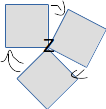
\includegraphics[width=0.25\textwidth]{aufgabe1a}} 
	\end{figure} 

Wir überlegen uns nun, für welche Werte von $m$ die genannte Forderung eingehalten 
werden kann. Dazu schauen wir uns an, wie groß der Innenwinkel einer Ecke 
eines $m$-Ecks ist. Für einfache n-Ecke gibt $(n-2)*180^{\circ}$ die Innenwinkelsumme an.
Da wir regelmäßige $m$-Ecke gegeben haben, ist die Größe eines Innenwinkels eines
regelmäßigen $m$-Ecks mit $\frac{(m-2)*180^{\circ}}{m}$ gegeben. Entsprechend gibt 
nun folgende Funktion an, wie viele $m$-Ecke wir maximal überlappungsfrei um eine zentrale Ecke $z$
im Kreis anordnen können: $f(m) = \frac{360^{\circ}}{\frac{(m-2)*180^{\circ}}{m}} = 
\frac{360^{\circ} * m}{(m-2) * 180^{\circ}} = \frac{2m}{m-2}$.

Wegen $f'(m) = -\frac{4}{(m-2)^2}$ ist $f(m \in (2,\infty))$ streng monoton fallend. 
Da wir in jedem Fall minimal 3 $m$-Ecke überlappungsfrei anordnen können müssen, 
setzen wir $f(m) = 3$ und erhalten $\frac{2m}{m-2} = 3 \Leftrightarrow m = 6$.
Das reguläre 6-Eck ist also das "`maximale"' $m$-Eck, bei dem wir gerade noch 3 
$m$-Ecke überlappungsfrei im Kreis um eine zentrale gemeinsame Ecke $z$ anordnen können.
Da wir jedoch wie beschrieben, zusätzlich jeweils eine Kante zweier $m$-Ecke
 mit Endpunkt in $z$ benötigen, welche aufgrund der Distanz nicht miteinander
 verbunden/zur Deckung gebracht werden können, muss gelten $f(m) > 3$.
 Das $m$-Eck mit $m = 6$ Ecken scheidet daher als Kandidat für einen platonischen Körper aus.
 Es verbleiben deshalb noch die "`Kandidaten"' $m = 3$, $m = 4$ und $m = 5$.
 Für $m = 5$ erhalten wir $f(5) = \frac{10}{3} = 3,\overline{3}$. Wir können also
 genau \textbf{3 5-Ecke} entsprechend um ein Zentrum $z$ anordnen und haben wegen des "`überlappenden"'
 Nachkommawertes von $0,\overline{3}$ entsprechende zwei Kanten die nicht mehr verbunden werden können.
 Für $m = 4$ sind entsprechend $f(4) = \frac{8}{2} = 4$ 4-Ecke um $z$ möglich, jedoch wieder ohne
 Nachkommastelle. Deshalb kann es nur noch den nächst niedrigeren Wert von \textbf{3 4-Ecken} geben.
 Für $m = 3$ erhalten wir $f(3) = \frac{6}{1} = 6$. Wegen der fehlenden Nachkommastelle, 
 erhalten wir wieder nur die nächst niedrigeren möglichen Werte von \textbf{5, 4 und 3 für m = 3}. 
 
 Insgesamt gibt es also höchstens die folgenden 5 Möglichkeiten eines platonischen Körpers:
 
 \begin{itemize}
 	\item 3 5-Ecke bilden eine Ecke  (existiert und wird "`Dodekaeder"' genannt)
 	\item 3 4-Ecke bilden eine Ecke  (existiert und wird "`Hexaeder"' genannt)
 	\item 5 3-Ecke bilden eine Ecke  (existiert und wird "`Ikosaeder"' genannt)
 	\item 4 3-Ecke bilden eine Ecke  (existiert und wird "`Oktaeder"' genannt)
 	\item 3 3-Ecke bilden eine Ecke  (existiert und wird "`Tetraeder"' genannt)
 \end{itemize}
 
 Wie wir in der Literatur nachschlagen können, sehen wir, dass diese Möglichkeiten 
 in Form der aufgeführten Bezeichnungen auch wirklich existieren.
  

\subsection*{(b)}
Was ist mit "`geometrische Graphen"' gemeint? 
Wenn man beim Dodekaeder die Mittelpunkte benachbarter Flächen verbindet erhält man
das Ikosaeder. Ist dies damit gemeint?

\section*{Aufgabe 2 - d-dimensionale Polytope}

\subsection*{(a)}
Die Ecken $W_{c(d)}$ eines d-dimensionalen Einheitswürfels $W_d$ sind gegeben mit

$W_{c(d)}=\{(x_1, ..., x_d) \in \mathcal{R}^d : x_1, ..., x_d \in \{0, 1\}\}$, 
wobei gilt $|W_{c(d)}| = 2^d$.

Sei $I \in \mathcal{R}^{d x d}$ die $d$-dimensionale Einheitsmatrix, 
$\vec{0}_d$ der d-dimensionale 0-Vektor und $\vec{1}_d$ der d-dimensionale
1-Vektor.

Dann sind die $d-1$-dimensionalen Facetten $W_{f_{d-1}(d)}$ von $W_d$ gegeben mit:

$W_{f_{d-1}(d)} = \{\vec{0}_d + x_1 e_{i1} + ... + x_{d-1} e_{i(d-1)}\} \cup \{\vec{1}_d - x_1 e_{i1} - ... - x_{d-1} e_{i(d-1)}\}$, wobei $x_i \in [0,1]$ und $e_{ij}$ Spaltenvektor von $I$.
Zudem muss für ein beliebiges aber festes $i$ gelten, dass die Vektoren $e_{ij}$ paarweise
verschieden sind. Und es muss für ein beliebiges aber festes $i_1$ 
und ein beliebiges aber festes $i_2$ mit $i_1 \neq i_2$ gelten: 
$\{e_{i_1j}\} \neq \{e_{i_2}j\}$.
Für die Größe von $W_{f_{d-1}(d)}$ gilt $|W_{f_{d-1}(d)}| = 2*d$.

\subsection*{(b)}
$W_4$ noch hierhin zeichnen... (https://de.wikipedia.org/wiki/4-D)

\subsection*{(c)}

\section*{Aufgabe 3 - Konvexe Hülle}

Die Punkte in S seien in allgemeiner Lage. Es wird die konvexe Hülle für $CH(S)$ gesucht. Wir nehmen an das $|S| = n$, wobei $n > 6$ ist. Der Fall $n \leq 6$ ist durch die allgemeine Lage von $S$ offensichtlich. Für $n > 6$:

\begin{enumerate}
	\item Es werden für alle Dimension die Extrempunkte $T  = \{x_{1_{min}}$, $x_{1_{max}}, \dots, x_{d_{min}}$, $x_{d_{max}}\}$ gesucht. Es wird ein Datenstruktur $F$ mit den Facetten des durch $T$ implizierten Octaeders angelegt. Des Weiteren wird der Schwerpunkt $g = \frac{\sum_{p \in T}{ p } }{|T|}$ berechnet. Die Menge $S = S \setminus T$ wird aktualisiert. Dies initiale Schritte liegen in $\mathcal{O}(n)$.
	\item Solange $S \neq \varnothing$:

	\begin{itemize}
		\item Wir wählen ein Punkt $p \in S$ und aktualisieren $S = S \setminus p$ und erstellen ein Strecke $s = \overline{gp}$.
		
		\item Berechne die Menge aller geschnitten Flächen: $I = \{f \quad | \quad s \cap f \neq \varnothing, (s \cap f) \neq p, f \in F\}$. $I$ sei ein Queue. Dazu prüfen wir iterativ alle Facetten in $F$ also $\mathcal{O}(n)$. Für die weitere Betrachtung nehmen wir an, dass das innere der konvexen Hülle als der Schnitt der negativen Halbräume aller
		durch die Flächen $f \in F$ definierten Ebenen gegeben ist.
		
		TODO: $|I| > 1$ wenn Strecke s eine Kante oder Ecke schneidet
		
		\item Fall $p \in CH(T)$ ist die Menge $I = \varnothing$, weiter mit Punkt zwei.
		\item Fall $p \notin CH(T)$ ist die Menge $I \neq \varnothing$. 
		\begin{itemize}
			\item Betrachte alle Nachbarn von $I$ und füge die Nachbarn zu $I$ hinzu, wenn $p$ im positiven Halbraum vom jeweiligen Nachbarn liegt. Falls ein Nachbar $r$ im negativen
Halbraum liegt, markiere genau die Kante, welche $r$ mit seinem Nachbarn in $I$ teilt. Dies wird solange wiederholt bis kein Nachbar $r$ mehr existiert, für den gilt, $p$ liegt im positiven Halbraum von $r$.  Die Laufzeit liegt $\mathcal{O}(n)$. 
			\item  Solange $I \neq \varnothing$
			\begin{itemize}
				\item Wähle $i = I.dequeue()$
				\item $F = triangulation(F,i,p)$ 
				\item Die drei Operation liegen in $\mathcal{O}(1)$.
			\end{itemize}
		\end{itemize}
		
	\end{itemize}		
\end{enumerate}

Die Funktion $triangulation(F,i,p)$ wird wie folgt definiert:

\begin{itemize}
	\item $F = F \setminus i$
	\item 
	\item Fall $i = I_1$: $F = F \cup \Delta_{i,p}$, wobei $\Delta_{i,p}$ die Menge aller Dreiecke der Triangulierung von $p$ mit der Facette $i$ ist.
	\item Sonst: 
\end{itemize}

Idee: (keine Ahnung, ob dies noch ein Brute-Force-Algo ist..
Nehme Extremwerte für x, y, z , und verbinde diese, 
dann hat man eine Art Octaeder, nur mit "`verzogenen"' Dreiecken als Flächen, also nicht regelmäßig..


Berechne den Schwerpunkt $s$ durch akkumulieren der Extremwerte und Division durch 6.

Ab jetzt für jeden neuen Punkt $p$:

\begin{itemize}
	\item Teste für alle aktuell bekannten begrenzenden Flächen (am Anfang die 8
	beschriebenen Dreiecke), welche die Strecke
	von $\overline{sp}$ schneidet. 
	\item Falls kein Schnitt mit irgendeiner der Flächen (Dreiecke) existiert fahre mit dem nächsten Punkt fort
	\item Falls ein Schnittpunkt $i$ mit Fläche $f$ existiert, ersetze $f$ (1 Dreieck) durch
	die neu entstehenden 3 Flächen (neue 3 Dreiecke), welche alle in der neuen Ecke $p$
	zusammenlaufen.. (alle bekannten Flächen zu jedem Zeitpunkt in $F$ gespeichert. )
\end{itemize}

Laufzeit:

Finden der Extremwerte geht in O(n).

Testen aller Flächen auf einen Schnitt mit der Strecke $\overline{sp}$ geht in O(1) *
O(aktuelle Anzahl der Flächen in $F$)

Also, wenn für jeden neuen Punkt $p$ neue Flächen entstehen (also 3 pro Punkt) , 
müssen in jedem Schritt 3 neue Flächen hinzugefügt werden und entsprechend steigt
die Zeit für die Überprüfung auf einen Schnitt in den nächsten Schritten..
Insgesamt sowas wie 0($n^2$)..

\end{document}

